\documentclass{standalone}
\usepackage{tikz,tikz-3dplot}

\usetikzlibrary{math,shapes.geometric}

\begin{document}

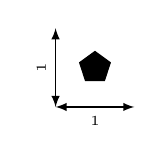
\begin{tikzpicture}
  \node[regular polygon,regular polygon sides=5,draw,fill=black] at (0.5,0.5) {};
  \draw[latex-latex] (0,0) -- ++(1,0) node [midway,below,font=\tiny] {1};
  \draw[latex-latex] (0,0) -- ++(0,1) node [midway,above,sloped,font=\tiny] {1};
\end{tikzpicture}

\end{document}
